\documentclass[a4paper]{article}
\usepackage[utf8]{inputenc}
\usepackage{fullpage} % Package to use full page
\usepackage{parskip} % Package to tweak paragraph skipping
\usepackage{tikz} % Package for drawing
\usepackage{listings}
\usepackage{amsmath}
\usepackage{hyperref}
\usepackage{cleveref}
\usepackage{subcaption}

\title{{\small 02427 Advanced Time Series Analysis E18}\\Computer exercise 3}
\author{Niklas Christoffer Petersen}
\date{2018-11-07}

\begin{document}

\maketitle

\section{Part 1}

\subsection{Question 1a}

\begin{figure}[ht!]
    \centering
    \begin{subfigure}[b]{0.45\textwidth}
        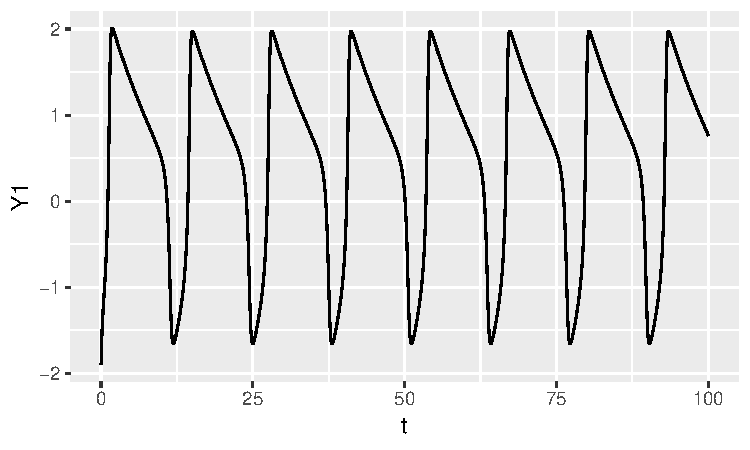
\includegraphics[width=\textwidth]{part1a-sigma0-Y1.pdf}
        \caption{$Y^1$}
    \end{subfigure}
    ~
    \begin{subfigure}[b]{0.45\textwidth}
        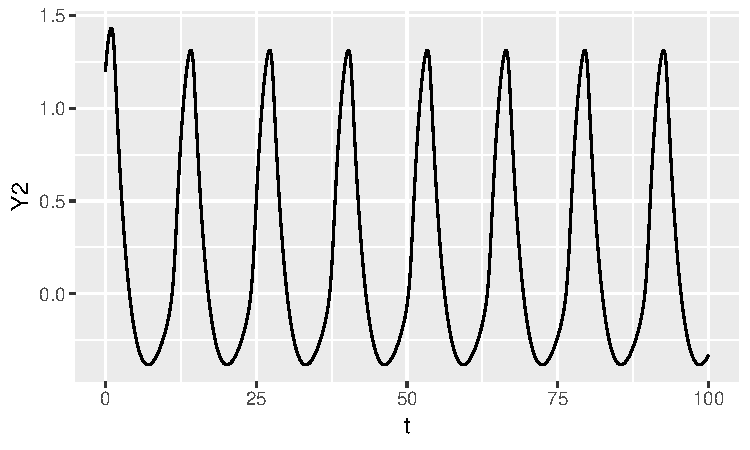
\includegraphics[width=\textwidth]{part1a-sigma0-Y2.pdf}
        \caption{$Y^2$}
    \end{subfigure}
    \caption{Realized values of $Y^1$ amd $Y^2$ for $\sigma = 0$}\label{fig:part1a-sigma0}
\end{figure}

\begin{figure}[ht!]
    \centering
    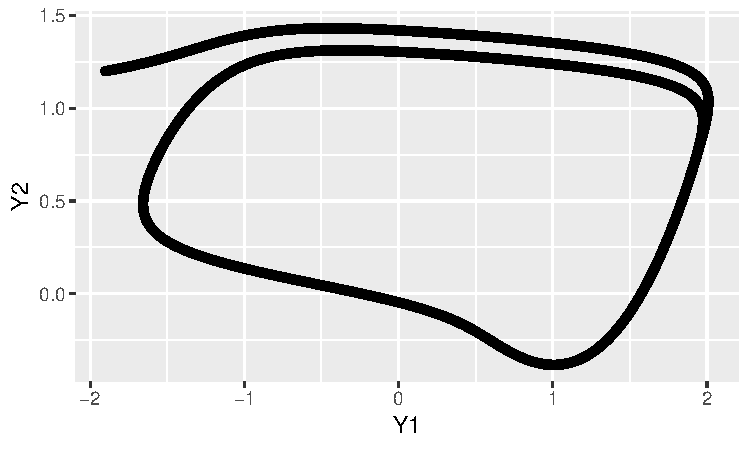
\includegraphics[width=\textwidth]{part1a-sigma0-Y1Y2.pdf}
    \caption{Phase Plot $Y^1$ amd $Y^2$ for $\sigma = 0$}\label{fig:part1a-sigma0-Y1Y2}
\end{figure}


\clearpage
\begin{figure}
    \centering
    \begin{subfigure}[b]{0.45\textwidth}
        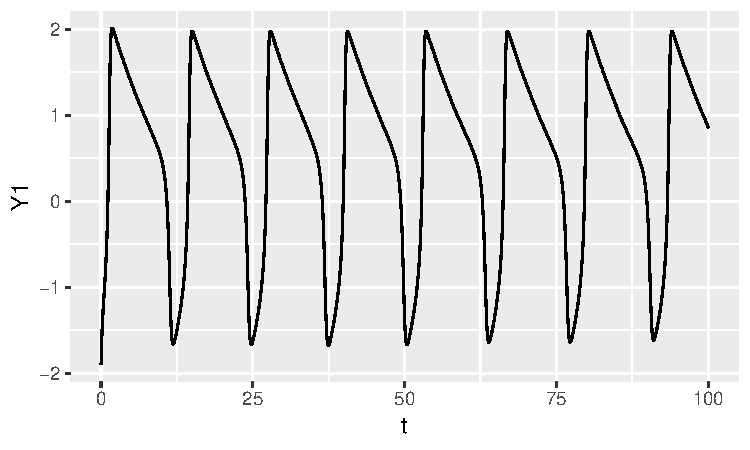
\includegraphics[width=\textwidth]{part1a-sigma1-Y1.pdf}
        \caption{$Y^1$}
    \end{subfigure}
    ~
    \begin{subfigure}[b]{0.45\textwidth}
        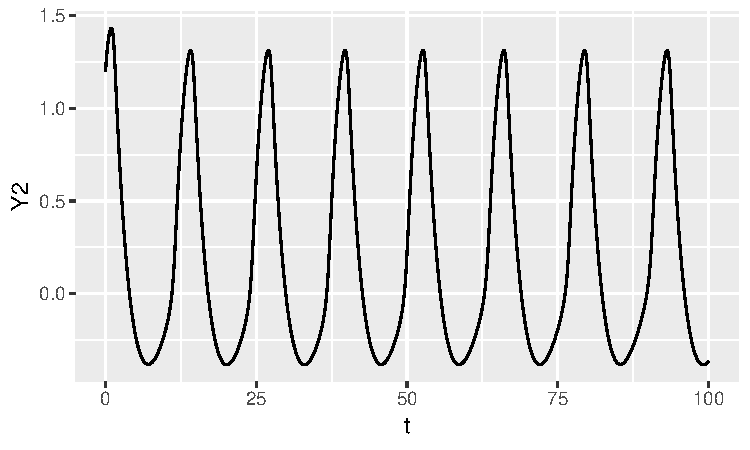
\includegraphics[width=\textwidth]{part1a-sigma1-Y2.pdf}
        \caption{$Y^2$}
    \end{subfigure}
    \caption{Realized values of $Y^1$ amd $Y^2$ for $\sigma = 0.10$}\label{fig:part1a-sigma1}
\end{figure}
\begin{figure}
    \centering
    \begin{subfigure}[b]{0.45\textwidth}
        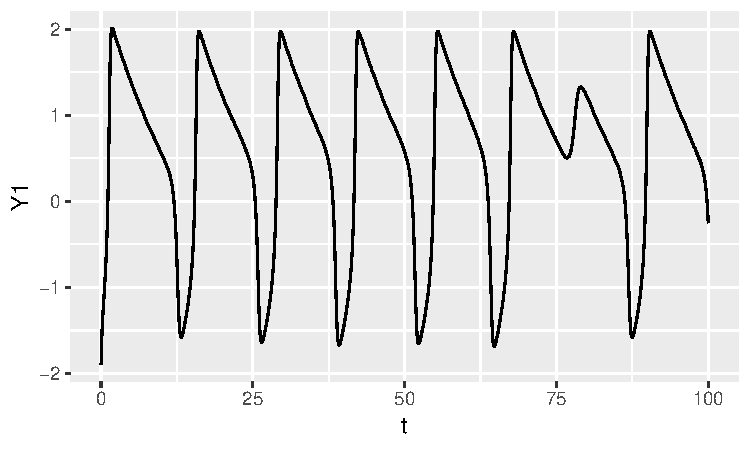
\includegraphics[width=\textwidth]{part1a-sigma2-Y1.pdf}
        \caption{$Y^1$}
    \end{subfigure}
    ~
    \begin{subfigure}[b]{0.45\textwidth}
        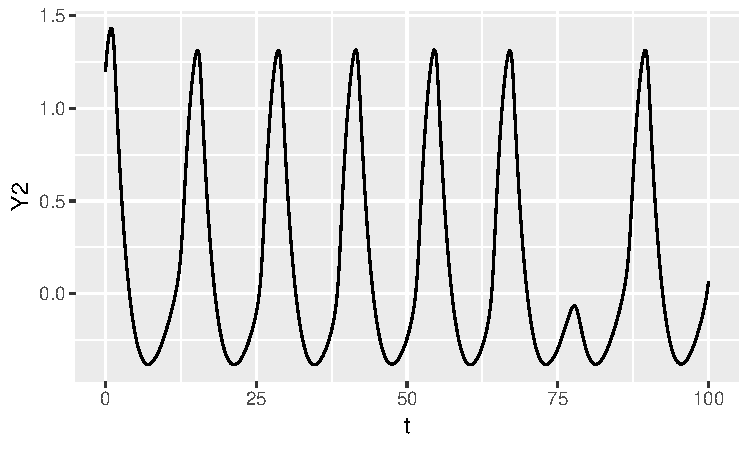
\includegraphics[width=\textwidth]{part1a-sigma2-Y2.pdf}
        \caption{$Y^2$}
    \end{subfigure}
    \caption{Realized values of $Y^1$ amd $Y^2$ for $\sigma = 0.20$}\label{fig:part1a-sigma2}
\end{figure}
\begin{figure}
    \centering
    \begin{subfigure}[b]{0.45\textwidth}
        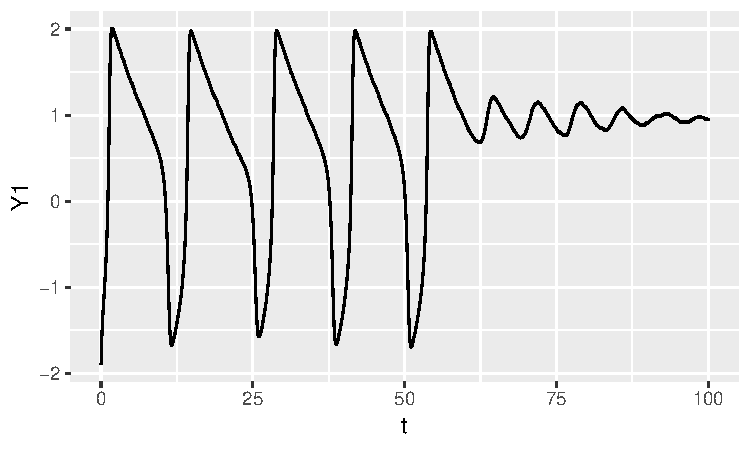
\includegraphics[width=\textwidth]{part1a-sigma3-Y1.pdf}
        \caption{$Y^1$}
    \end{subfigure}
    ~
    \begin{subfigure}[b]{0.45\textwidth}
        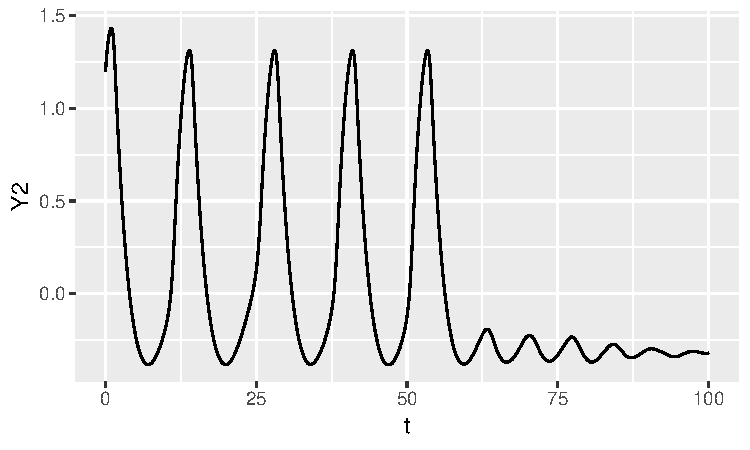
\includegraphics[width=\textwidth]{part1a-sigma3-Y2.pdf}
        \caption{$Y^2$}
    \end{subfigure}
    \caption{Realized values of $Y^1$ amd $Y^2$ for $\sigma = 0.30$}\label{fig:part1a-sigma3}
\end{figure}
\begin{figure}
    \centering
    \begin{subfigure}[b]{0.45\textwidth}
        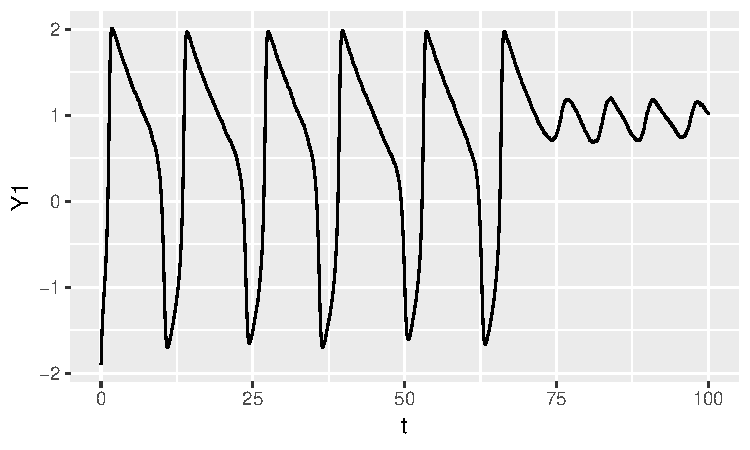
\includegraphics[width=\textwidth]{part1a-sigma4-Y1.pdf}
        \caption{$Y^1$}
    \end{subfigure}
    ~
    \begin{subfigure}[b]{0.45\textwidth}
        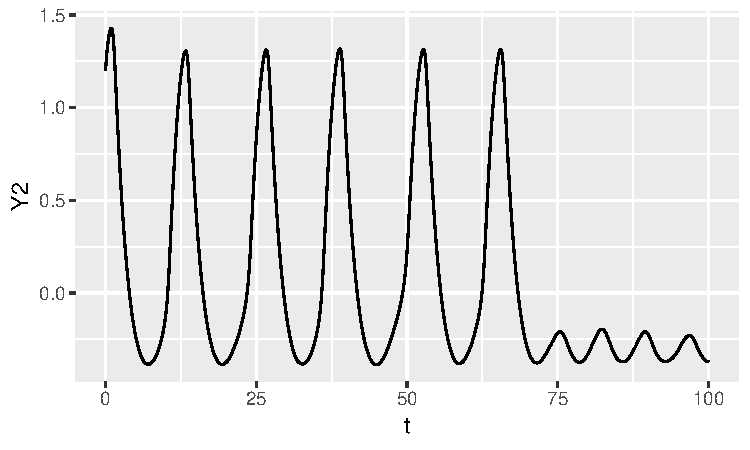
\includegraphics[width=\textwidth]{part1a-sigma4-Y2.pdf}
        \caption{$Y^2$}
    \end{subfigure}
    \caption{Realized values of $Y^1$ amd $Y^2$ for $\sigma = 0.40$}\label{fig:part1a-sigma4}
\end{figure}
\clearpage

\subsection{Question 1b}

\clearpage
\begin{figure}
    \centering
    \begin{subfigure}[b]{0.45\textwidth}
        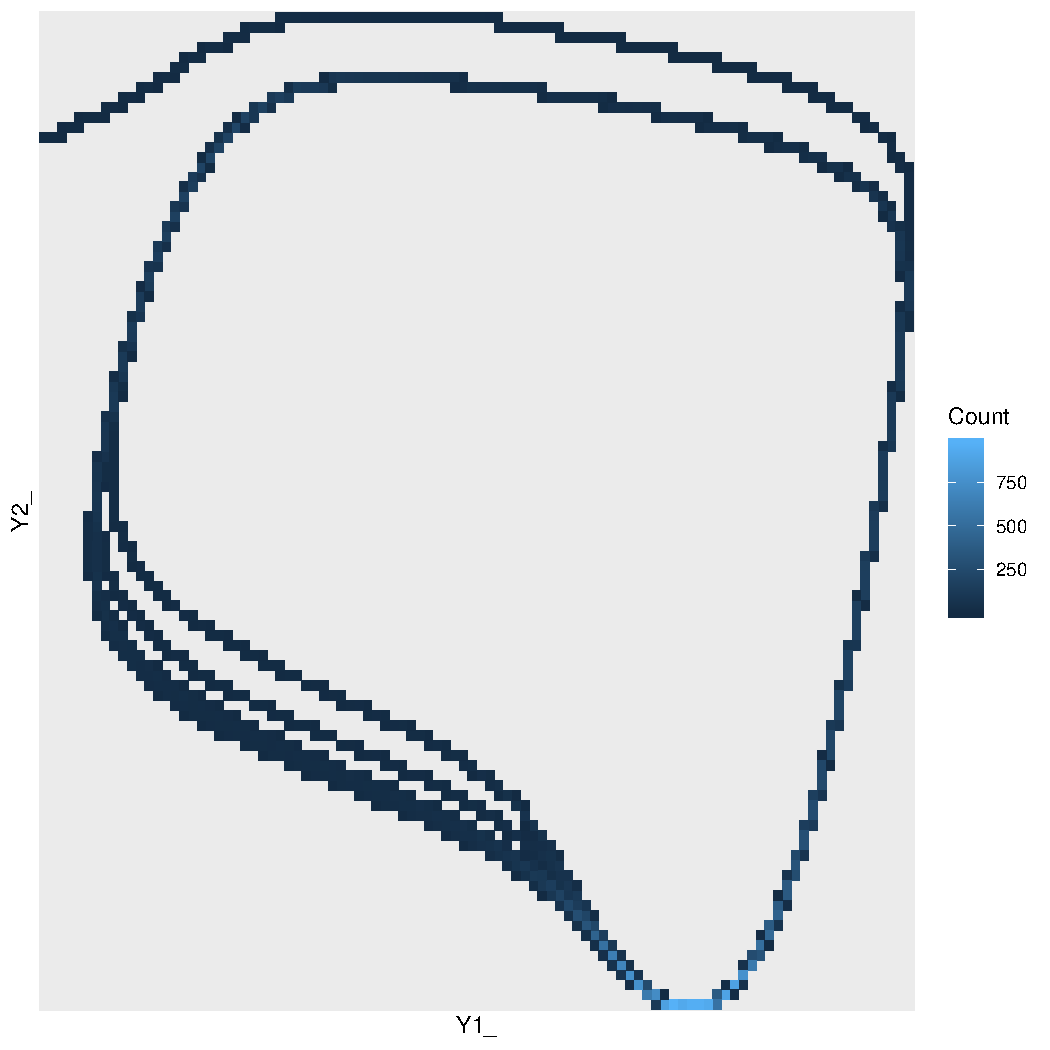
\includegraphics[width=\textwidth]{part1b-sigma1-grid.pdf}
        \caption{$Y^1$}
    \end{subfigure}
    ~
    \begin{subfigure}[b]{0.45\textwidth}
        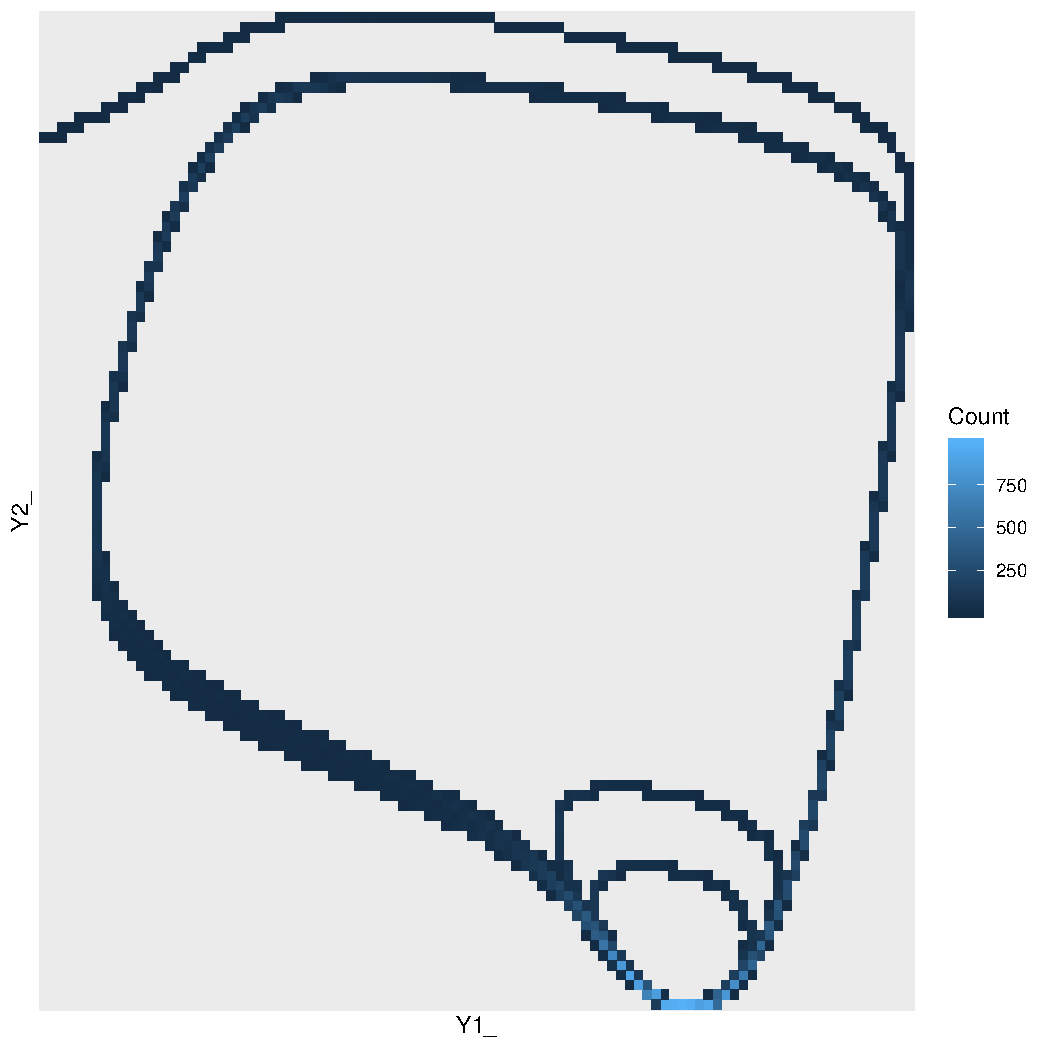
\includegraphics[width=\textwidth]{part1b-sigma2-grid.pdf}
        \caption{$Y^2$}
    \end{subfigure}
    ~
    \begin{subfigure}[b]{0.45\textwidth}
        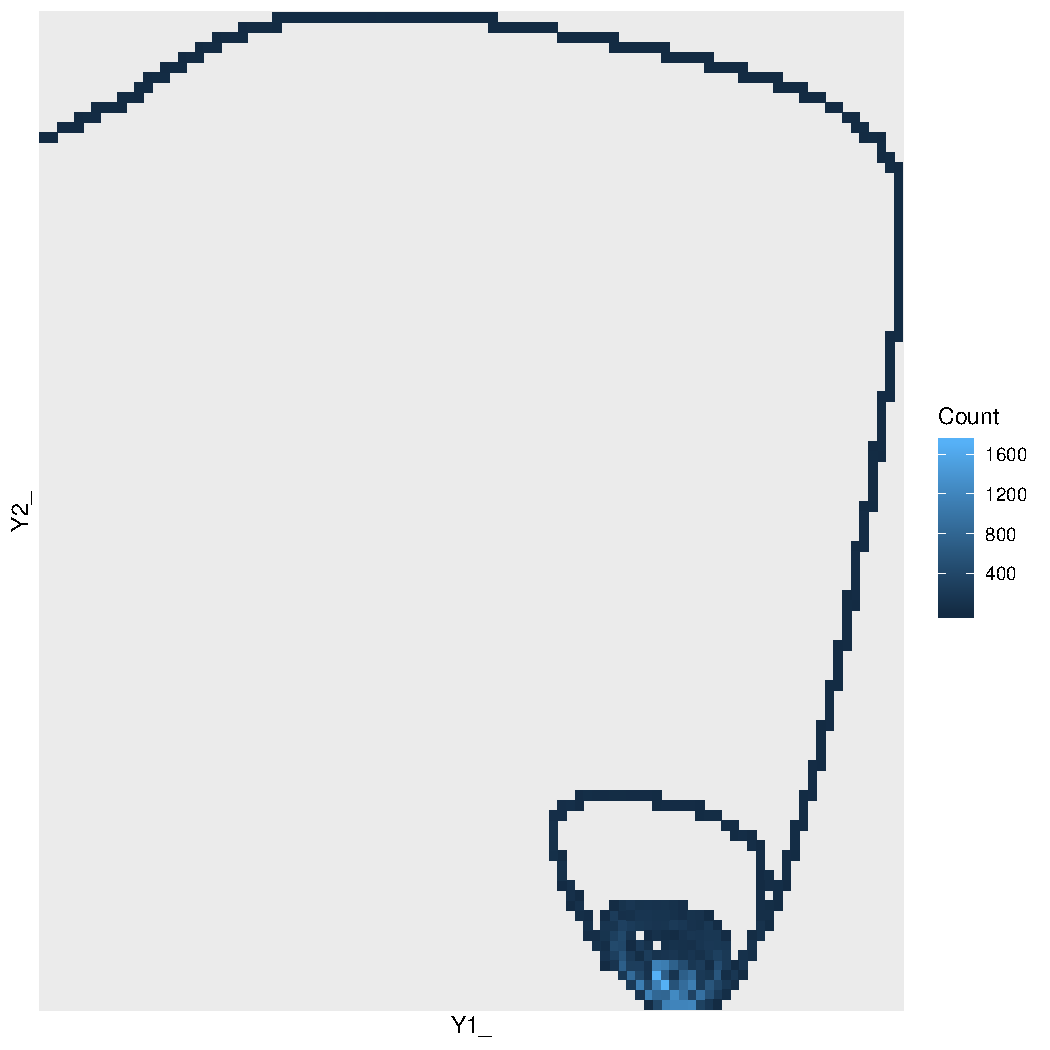
\includegraphics[width=\textwidth]{part1b-sigma3-grid.pdf}
        \caption{$Y^1$}
    \end{subfigure}
    ~
    \begin{subfigure}[b]{0.45\textwidth}
        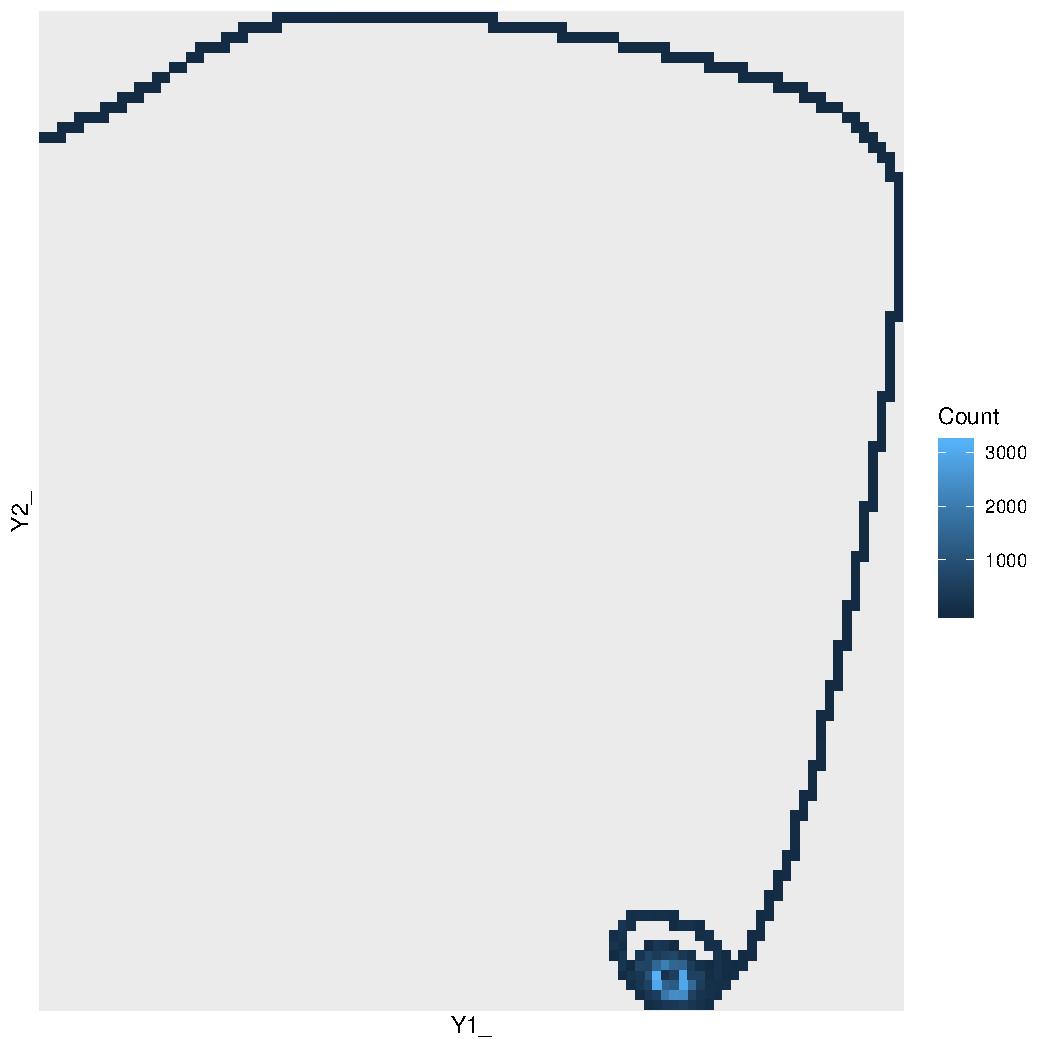
\includegraphics[width=\textwidth]{part1b-sigma4-grid.pdf}
        \caption{$Y^2$}
    \end{subfigure}
    \caption{Realized values of $Y^1$ amd $Y^2$ for $\sigma = 0.20$}\label{fig:part1a-sigma2}
\end{figure}
\clearpage

\section{Part 2}

We start our analysis with a exploration and some descriptive statistics of the source data.

\end{document}
